\section{\Acrfull{bsj} detection}

For detection of \gls{bsj}s, I used the five tools already introduced in
\cref{subsec:circrna_detection}.
As shown in \cref{fig:detection_bars}, find\_circ, CIRI2, DCC, and
circexplorer2 detect a similar number of \gls{bsj}s, while segemehl detects
almost ten times as many \gls{bsj}s as its closest competitor, DCC.

\begin{figure}[ht] \centering

    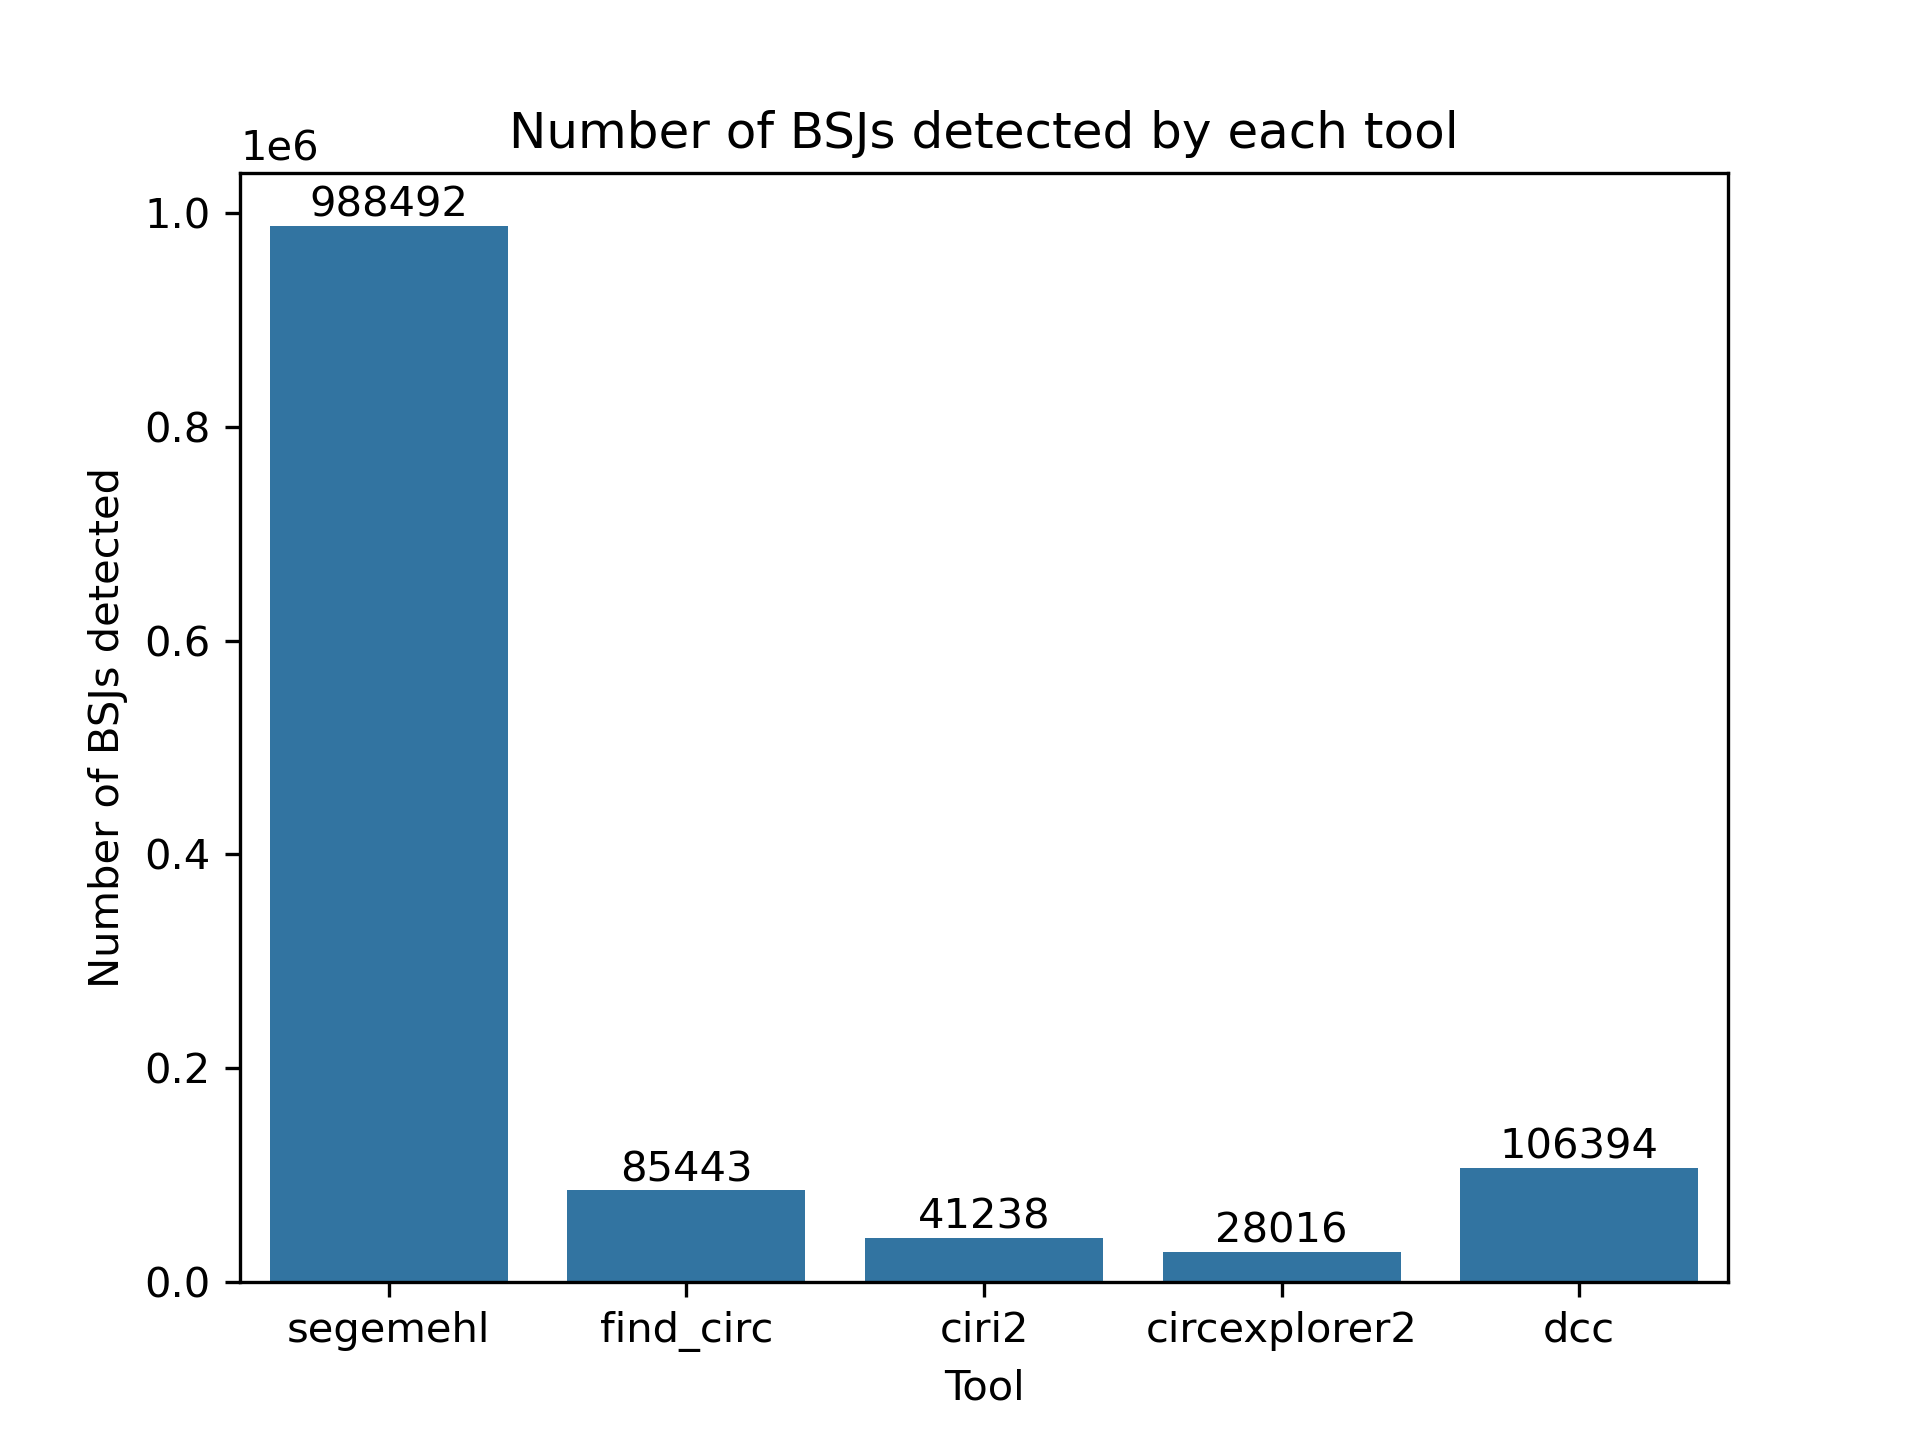
\includegraphics[width=0.6\textwidth]{chapters/4_results_and_discussion/figures/detection/n_bsjs_detected.png}
    \caption{Number of \gls{bsj}s detected by each tool.
        While find\_circ, CIRI2, DCC and circexplorer2 detect a similar number of
        \gls{bsj}s, segemehl detects a much larger number of \gls{bsj}s.
    }
    \label{fig:detection_bars}
\end{figure}
Similar behavior was previously observed by \textcite{zeng_comprehensive_2017},
where segemehl was among the top performers in terms of sensitivity, but also
had a high false positive rate.
The lowest numbers of \gls{bsj}s were detected by circexplorer2 and CIRI2,
which both have built-in filters to reduce false
positives\supercite{zhang_diverse_2016,gao_circular_2018}.

\subsection{Agreement between tools and the role of clustering}

% TODO: Why is agreement important?

To assess the agreement between the tools, I used UpSet plots, which show the
overlap of \gls{bsj}s detected by different tools.
When identifying the overlap between tools, the most strict approach is to
consider only \gls{bsj}s with identical start and end positions and on the same
strand as the same \gls{bsj}.
The according plot is shown in \cref{fig:detection_upset_0_strand}.
While there are a total of x \gls{bsj}s detected by at least two tools, only y
\gls{bsj}s are detected by three tools, and none are detected by four or five
tools.

When ignoring the strand information, the number of \gls{bsj}s detected by
three tools increases substantially, as shown in
\cref{fig:detection_upset_0_nostrand}.
Also the number of \gls{bsj}s detected by two tools increases, while still no
\gls{bsj}s are detected by four or five tools.

When exploring the data, I noticed that there are many detected \gls{bsj}s that
are very close to each other, but not identical - thus not being counted as the
same \gls{bsj} when grouping in the conventional way.
In order to investigate this further, I introduced a more lenient grouping
criterion.
Here, both the start and end positions of the \gls{bsj}s are separately
clustered using single linkage clustering.
This means, a \gls{bsj} is considered to be part of a cluster if it is within a
certain distance of any other \gls{bsj}'s start/end position.
Two \gls{bsj}s are considered the same if they are part of the same cluster
regarding both their start and end positions.
In the following analysis, I will refer to the distance limit as the
\textit{shift}.

When allowing a shift of only 1 bp, the results change drastically.
As shown in \cref{fig:detection_upset_1_nostrand}, a large number of \gls{bsj}s
are detected by four and even five tools, while the number of \gls{bsj}s
detected by three tools decreases.

\begin{figure}[ht] \begin{tabular}{cc} \begin{subfigure}{.5\textwidth}
                                           \centering

                                           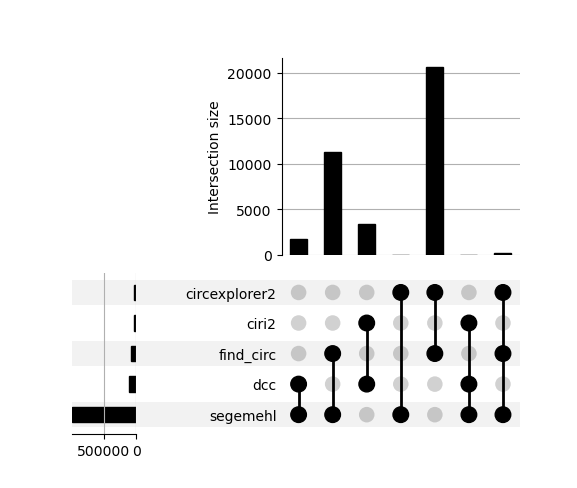
\includegraphics[width=\linewidth]{chapters/4_results_and_discussion/figures/detection/upset/diff_0_strand.png}
                                           \caption{No shift allowed, strand
                                               considered}
                                           \label{fig:detection_upset_0_strand}
                                       \end{subfigure} &
               \begin{subfigure}{.5\textwidth} \centering

                       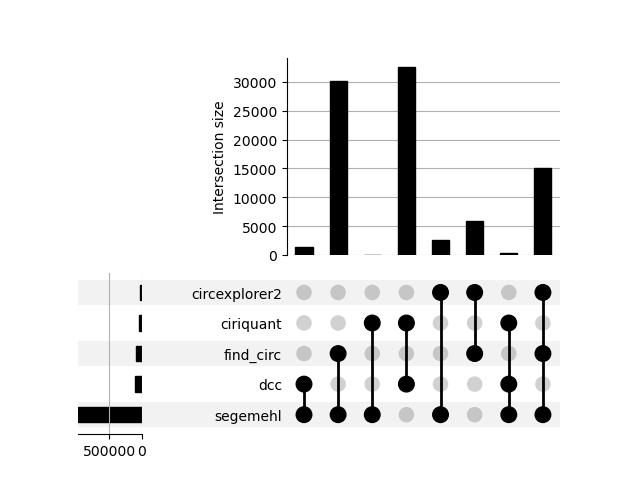
\includegraphics[width=\linewidth]{chapters/4_results_and_discussion/figures/detection/upset/diff_0_nostrand.png}
                       \caption{No shift allowed, strand ignored}
                       \label{fig:detection_upset_0_nostrand} \end{subfigure}
               \\ \multicolumn{2}{c}{
                   \begin{subfigure}{\textwidth} \centering

                           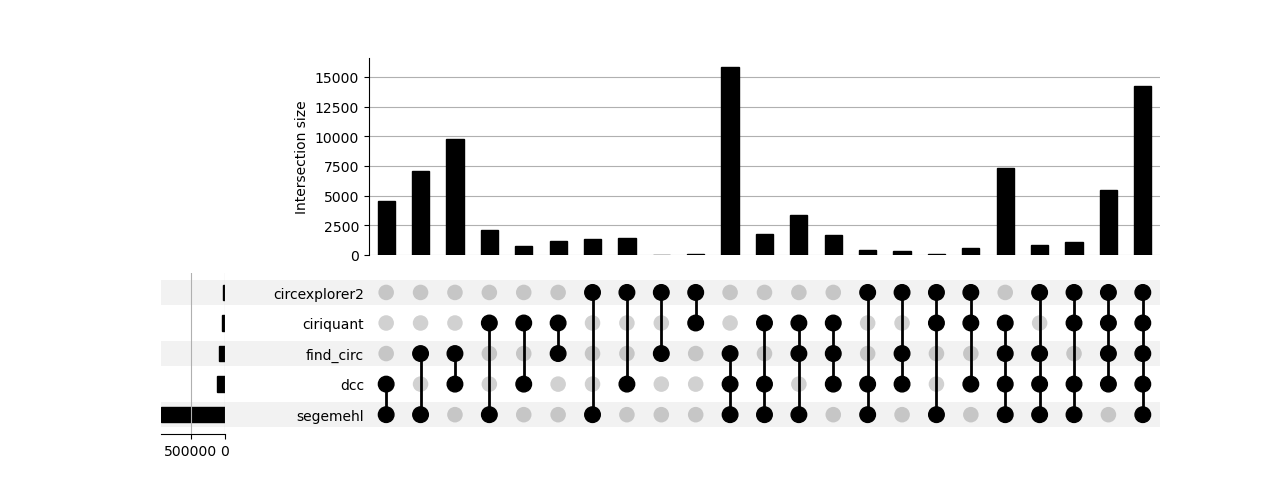
\includegraphics[width=\linewidth]{chapters/4_results_and_discussion/figures/detection/upset/diff_1_nostrand.png}
                           \caption{Shift of 1 allowed, strand ignored}
                           \label{fig:detection_upset_1_nostrand}

                       \end{subfigure}}\end{tabular} \caption{Upset plots
        showing the overlap of
        \gls{bsj}s detected by different tools using various grouping criteria.
        Only groups with at least two agreeing tools are displayed.
        When considering strand information and only counting \gls{bsj}s with identical
        start and end positions, many \gls{bsj}s are detected by just two tools, with
        very few detected by three tools (\cref{fig:detection_upset_0_strand}).
        Ignoring the strand information substantially increases the number of
        \gls{bsj}s detected by 3 tools (\cref{fig:detection_upset_0_nostrand}).
        Allowing a shift of 1 bp in the start and end positions while ignoring the
        strand information changes the results drastically, leading to a large number
        of \gls{crna}s with agreement between 4 and even 5 tools
        (\cref{fig:detection_upset_1_nostrand}).
    }
    \label{fig:detection_upset}
\end{figure}

As shown in \cref{fig:detection_upset_1_strand}, allowing a shift of 1 bp while
considering the strand information also leads to a number of \gls{bsj}s
detected by four and five tools, but the number is way lower than when ignoring
the strand information.
Increasing the allowed shift to larger values, e.g., 20 bp, does not lead to a
substantial change compared to the results when allowing a shift of 1 bp, as
shown in \cref{fig:detection_upset_20_nostrand}.

In my interpretation, the results show that in many cases the tools generally
agree on the detection of \gls{bsj}s, but the agreement is not perfect.
The fact that a shift of 1 bp leads to substantial changes while further
increasing the shift does not, indicates that in most cases the clustering
\gls{bsj}s form continuous chains between their start and end positions between
their extremes.
This suggests, that the tools are generally able to detect the back-spliced
reads, but have difficulties in determining the exact location of the
\gls{bsj}.

\subsection{Investigating the influence of the number of per-tool metrics on
    the agreement}

So far, the entire set of \gls{bsj}s detected by each tool was used for
investigation of agreement with other tools.
Now, I will investigate if the number of samples a \gls{bsj} was detected in
and the total number of reads supporting the \gls{bsj} across all samples
influences the agreement.
The plots in \cref{fig:detection_density} show the distribution of \gls{bsj}s
detected by each tool.

When looking at the distribution along the x-axis, it is apparent that all
tools have a large fraction of \gls{bsj}s detected in only a very small number
of samples.
While all tools have the lowest level of agreement in this region, after a
certain threshold the agreement becomes relatively stable and does not further
increase.

The mean count of reads supporting a \gls{bsj} across all samples where the
\gls{bsj} was detected is shown on the y-axis.
Here, the behavior of the tools is more heterogenous: While for CircExplorer2
and DCC the agreement increases with the mean read count, for CIRI2 and
find\_circ the opposite appears to be the case.

All tools have a small number of \gls{bsj}s with a very high mean read count.
For these, the agreement appears to be much lower, even if the \gls{bsj} is
detected in many samples.

\begin{figure}[ht] \begin{tabular}{cc} \begin{subfigure}{.4\textwidth}
                                           \centering 

                                           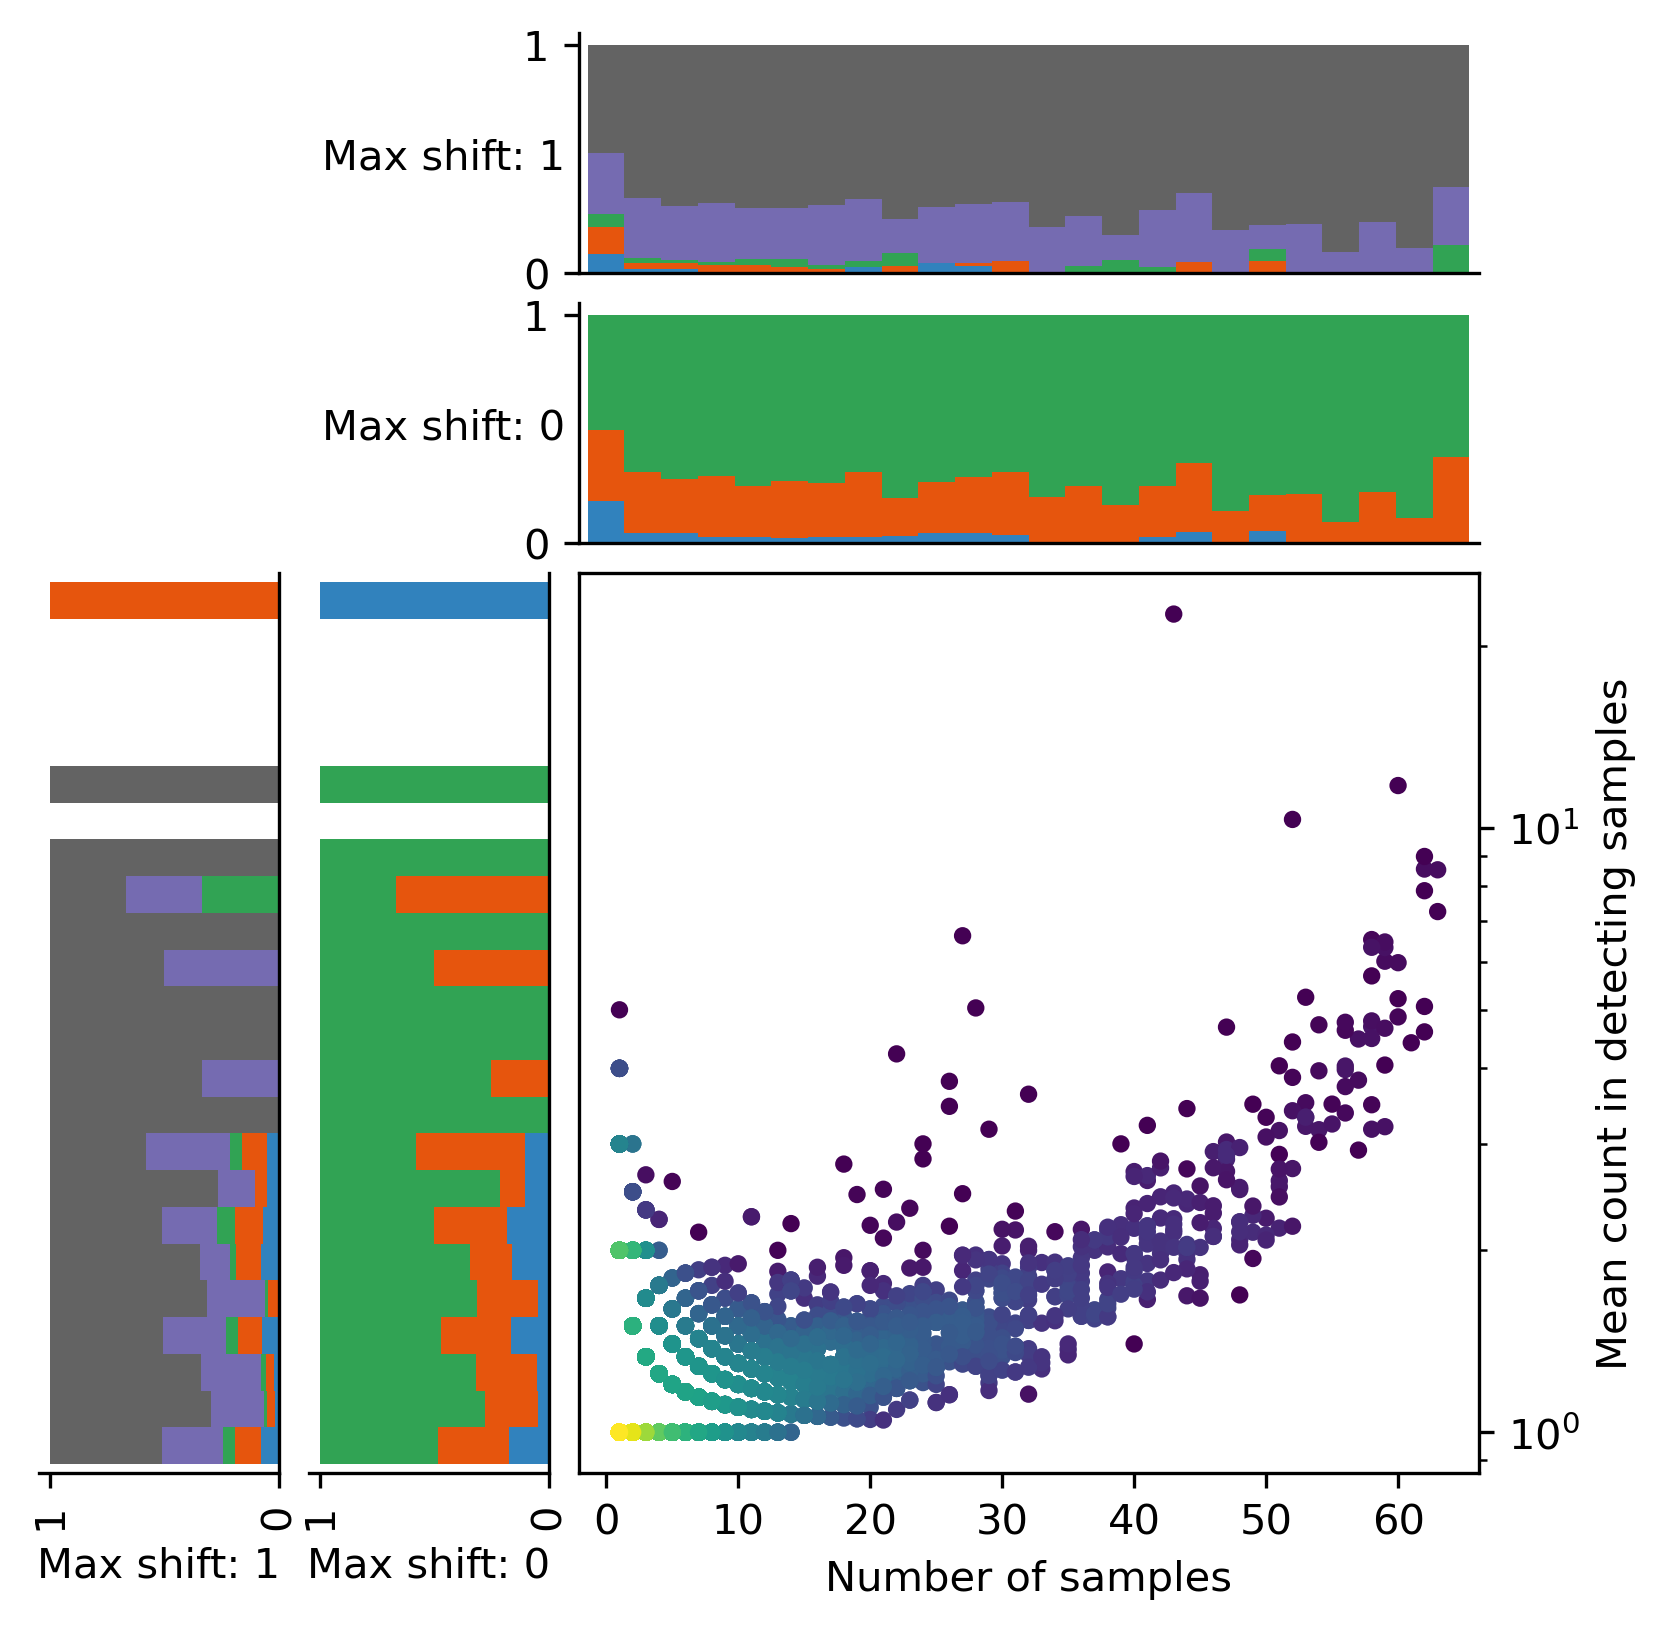
\includegraphics[width=\linewidth]{chapters/4_results_and_discussion/figures/detection/density/circexplorer2.png}
                                           \caption{CircExplorer2} 

                                           \label{fig:detection_density_circexplorer2} \end{subfigure} &
               \begin{subfigure}{.4\textwidth} \centering 

                       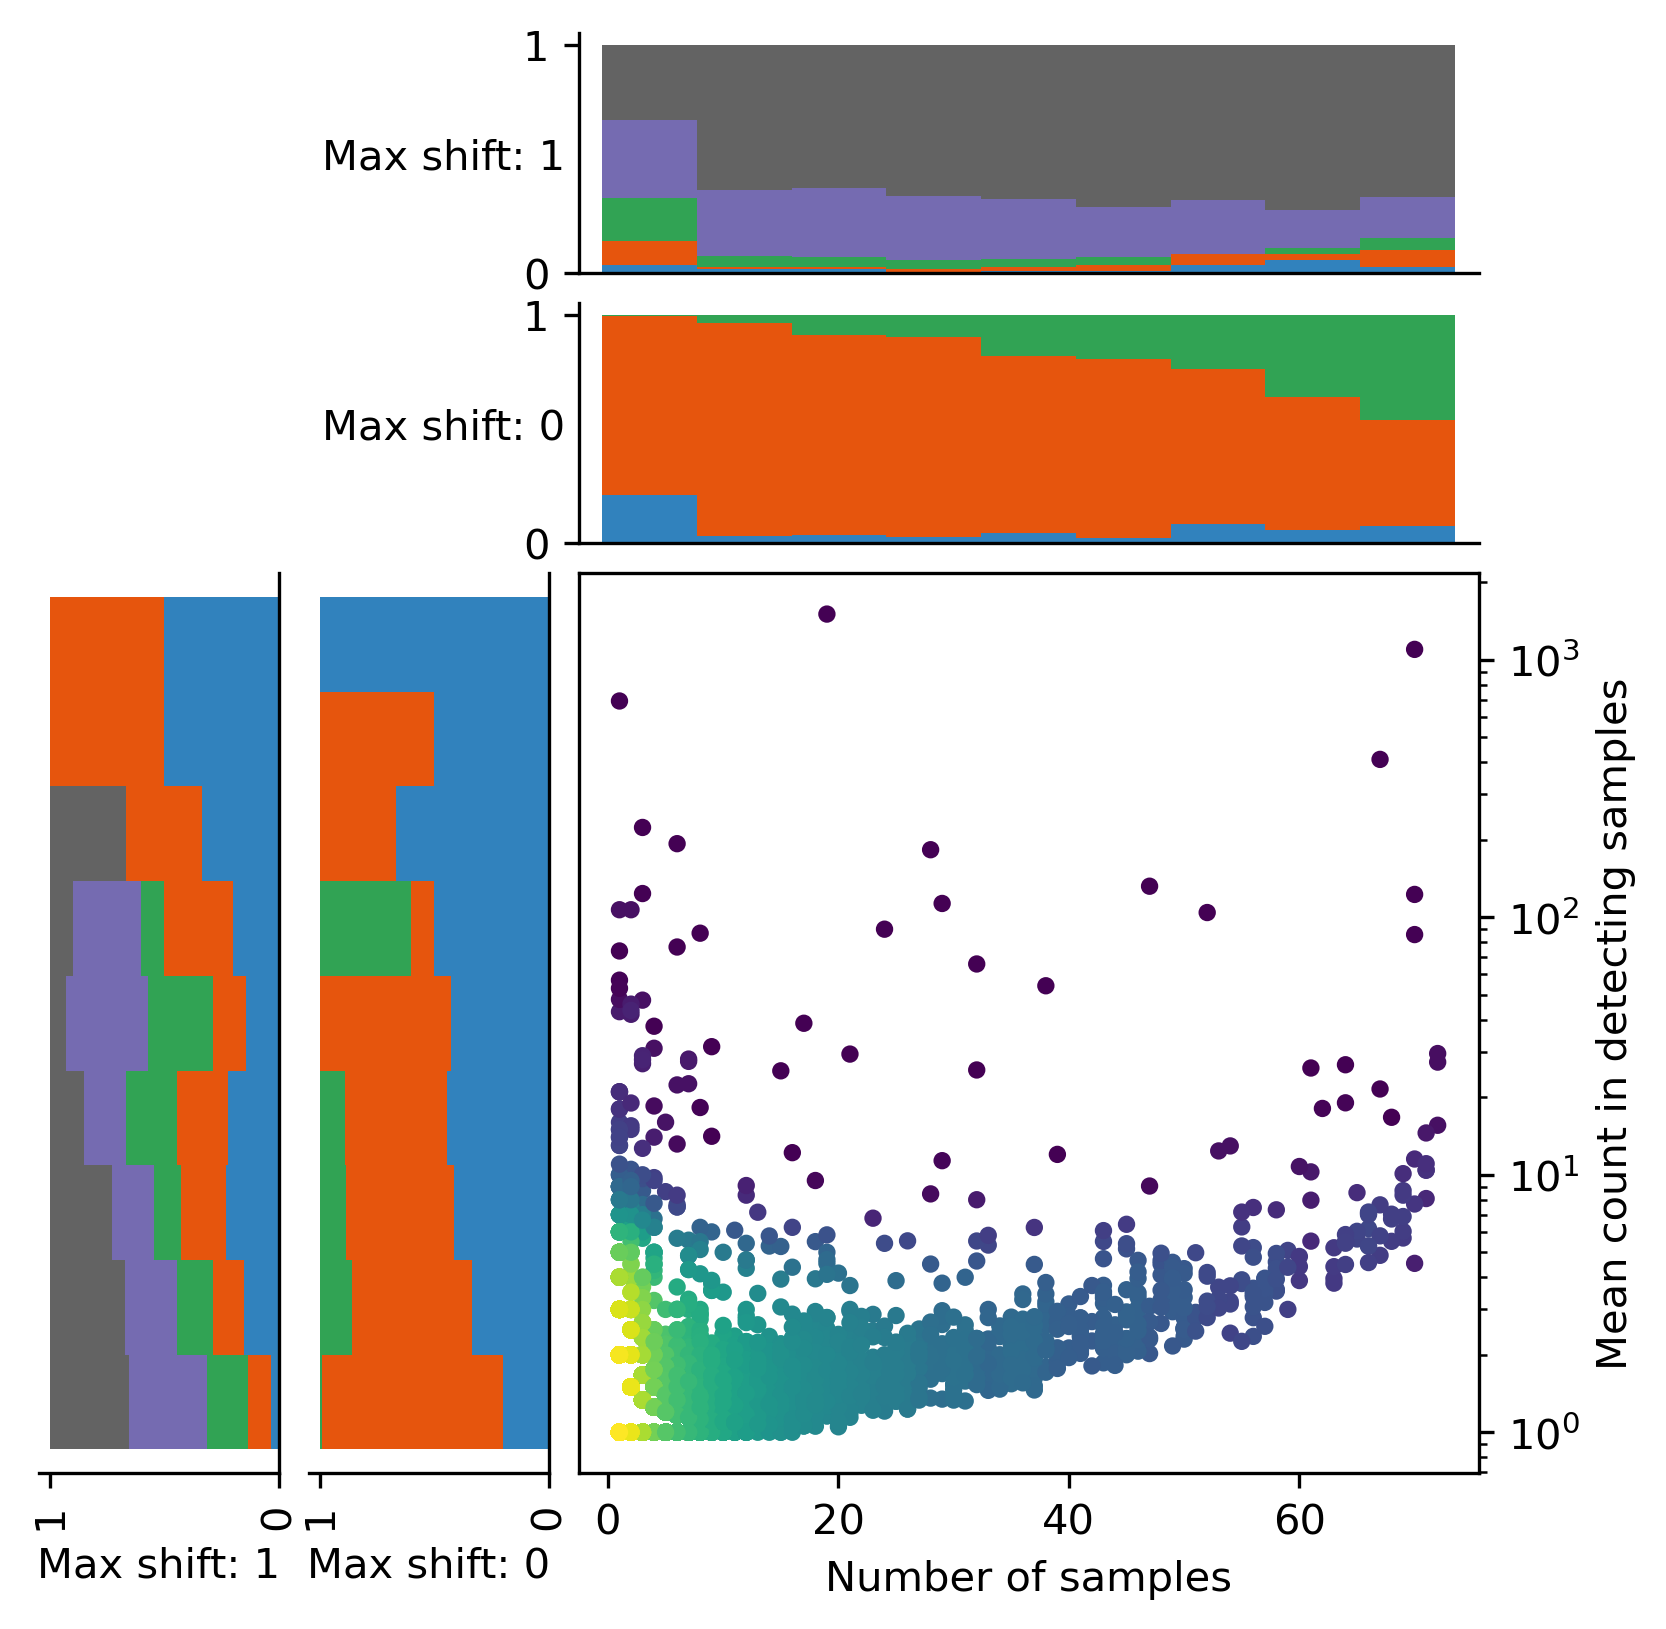
\includegraphics[width=\linewidth]{chapters/4_results_and_discussion/figures/detection/density/ciri2.png}
                       \caption{CIRI2} \label{fig:detection_density_ciri2} \end{subfigure}
               \\ \begin{subfigure}{.4\textwidth}
            \centering 

            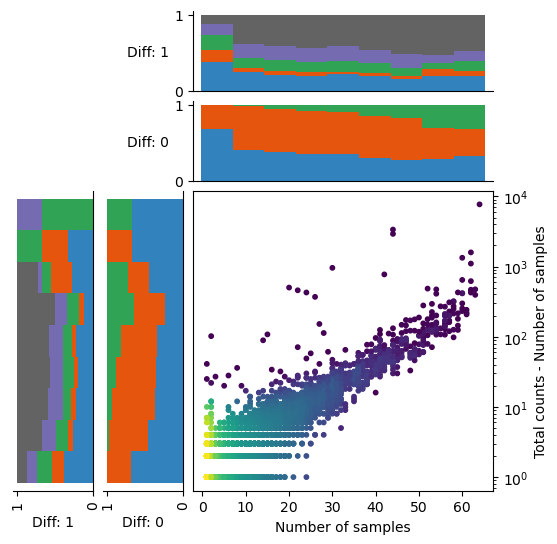
\includegraphics[width=\linewidth]{chapters/4_results_and_discussion/figures/detection/density/dcc.png}
            \caption{DCC} \label{fig:detection_density_dcc} \end{subfigure} &
                  \begin{subfigure}{.4\textwidth} \centering 

                       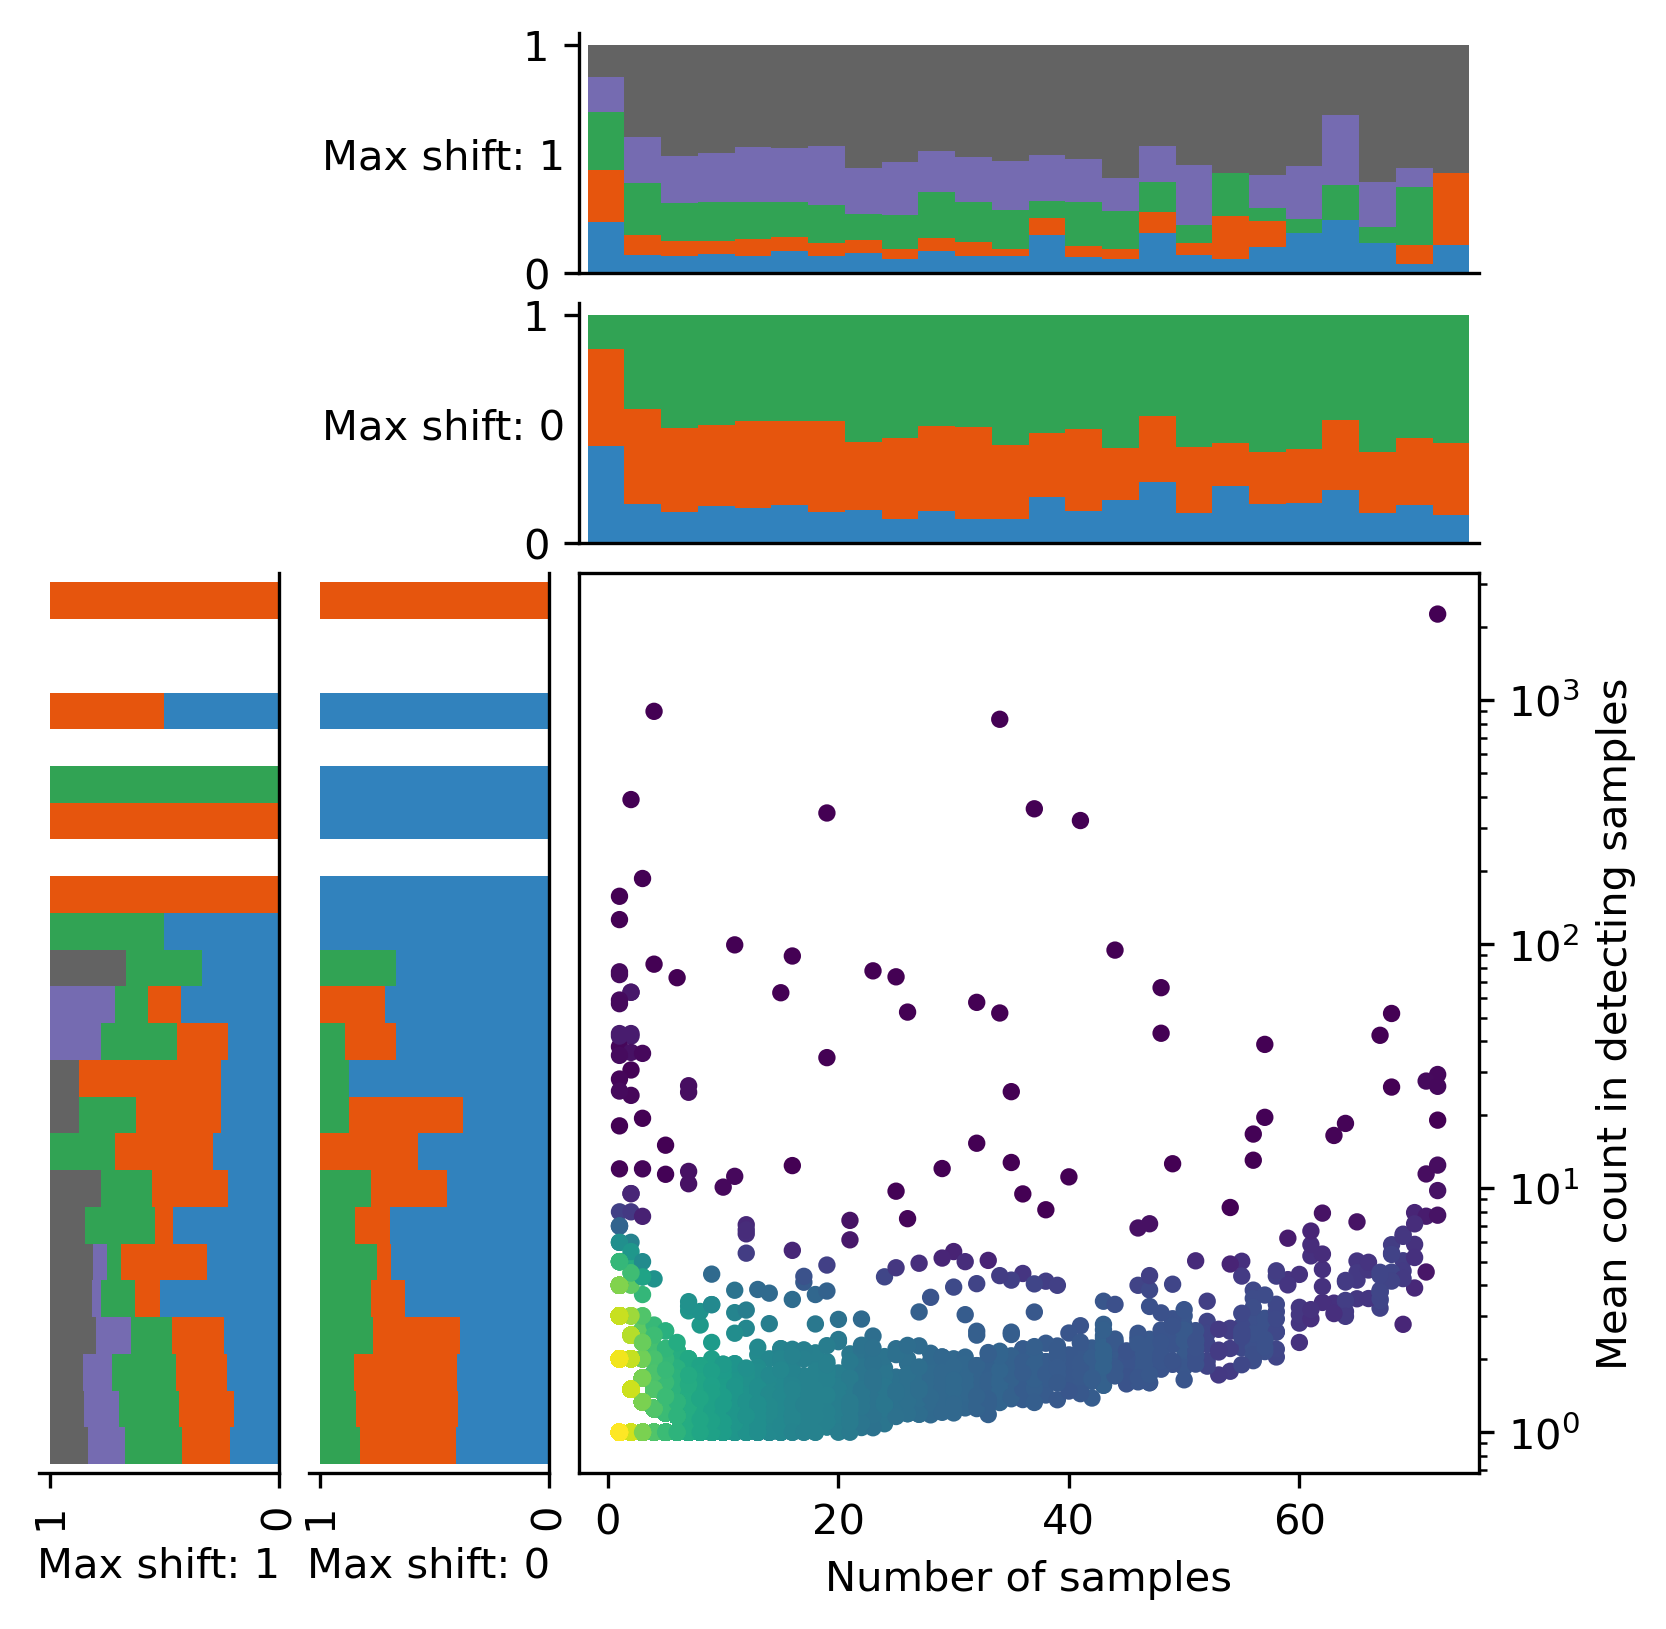
\includegraphics[width=\linewidth]{chapters/4_results_and_discussion/figures/detection/density/find_circ.png}
                       \caption{find\_circ} \label{fig:detection_density_find-circ} \end{subfigure}
               \\ \begin{subfigure}{.4\textwidth} \centering

            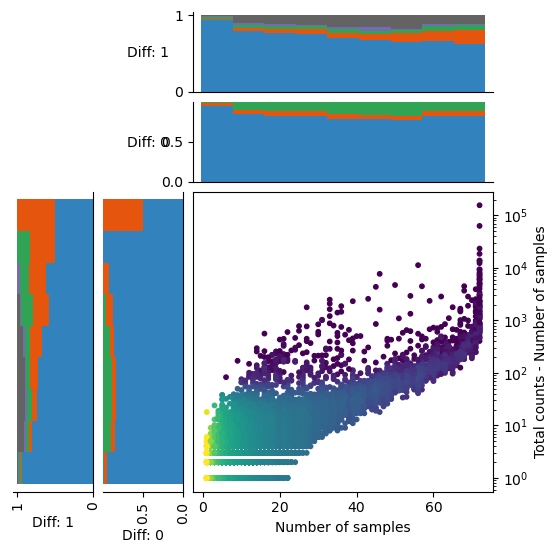
\includegraphics[width=\linewidth]{chapters/4_results_and_discussion/figures/detection/density/segemehl.png}
            \caption{Segemehl} \label{fig:detection_density_segemehl} \end{subfigure}

                                                                                                                                 & \begin{subfigure}{.4\textwidth}	 \centering \caption{Legend}

                                                                                                                                       \end{subfigure}\end{tabular} \caption{Distributions of \gls{bsj}s detected by
        each tool.
        % TODO: Add legend
        The x-axis shows the number of tools that detected a \gls{bsj}, while the
        y-axis shows mean number of reads supporting each \gls{bsj} across all samples
        where the \gls{bsj} was detected.
        The color indicates the logarithmized density of \gls{bsj}s at a given point.
        The stacked bar plots above and left of the scatter plots show the fraction of
        agreeing tools in the respective slice.
    }
    \label{fig:detection_density}
\end{figure}

\noindent\fbox{ \parbox{\textwidth}{ From now on, I will use the following
        filtering criteria: \begin{itemize} \item Clusters are formed by
                  grouping
                  \gls{bsj}s with a shift of 1 bp and ignoring the strand
                  information \item Only
                  \gls{bsj}s within clusters supported by at least four tools
                  are considered
        \end{itemize} } }


\subsubsection{Investigating the size of the intra-cluster distances}

In theory, the clustering process allows for the build-up of large clusters,
where the intra-cluster distance of both the start and end positions is large
compared to the minimum \gls{bsj} length derived from the maximum of the start
cluster and the minimum of the end cluster.

The terminology used here is illustrated in \cref{fig:clustering_expl}.

\begin{figure}[ht]
    \centering

    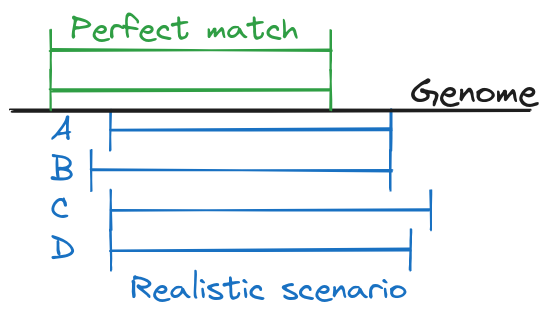
\includegraphics[width=0.7\textwidth]{chapters/4_results_and_discussion/figures/grouping.png}
    \caption{Schematic illustrating the terminology used in the
        clustering process}
    \label{fig:clustering_expl}
\end{figure}

\begin{figure}[ht]
    \begin{tabular}{cc}
        \begin{subfigure}{0.5\textwidth}
            \centering

            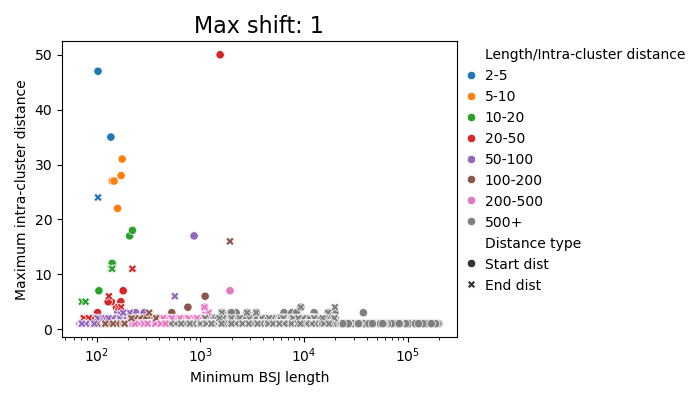
\includegraphics[width=\linewidth]{chapters/4_results_and_discussion/figures/detection/distances/diff_1_scatter.png}
            \caption{Relation between intra-cluster distance and \gls{bsj}
                length}
            \label{fig:clustering_scatter}
        \end{subfigure} &
        \begin{subfigure}{0.5\textwidth}
            \centering

            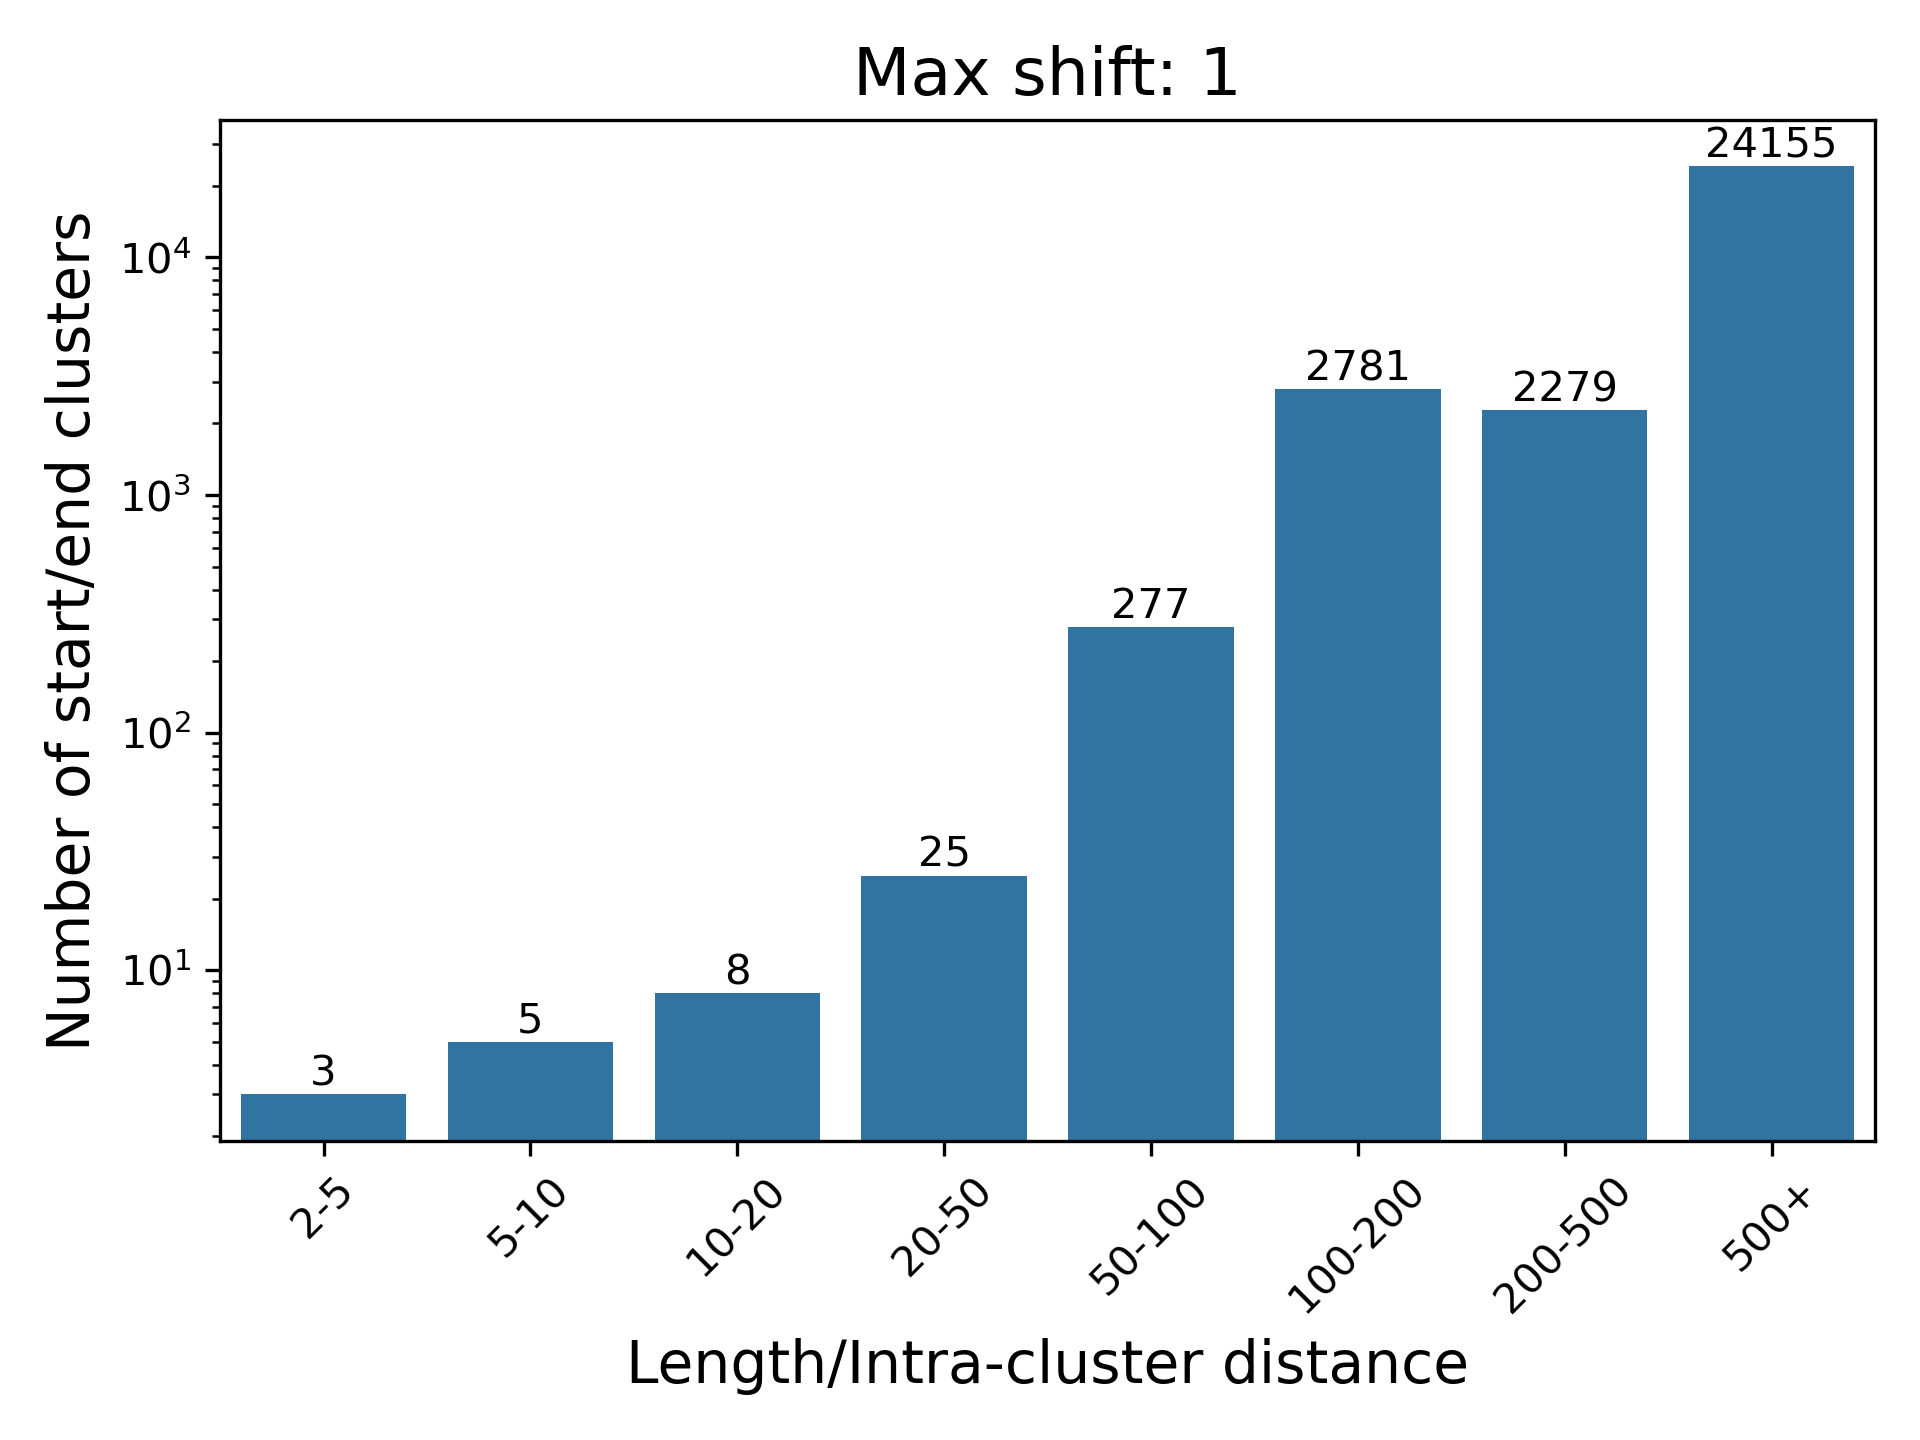
\includegraphics[width=\linewidth]{chapters/4_results_and_discussion/figures/detection/distances/diff_1_bar.png}
            \caption{Bar plot showing the number of clusters within a given
                ratio range}
            \label{fig:clustering_bar}
        \end{subfigure}
    \end{tabular}
    \caption{In order to investigate the relation between the intra-cluster
        distance and the minimum \gls{bsj} length the ratio between the two was
        used as a measure.
        The results show that the majority of clusters have a ratio of 50 or higher.
    }
    \label{fig:clustering}
\end{figure}

In order to investigate this further, I calculated the ratio between the
intra-cluster distances and the minimum \gls{bsj} length.
The results of this analysis are shown in \cref{fig:clustering_scatter}.
While there are 41 clusters with a ratio of 20 or lower, the vast majority of
clusters have a ratio of 50 or higher (indicating that for an intra-cluster
distance of 2, the \gls{bsj} must span at least 100 bp).
